\documentclass[12pt, letterpaper]{article}
\usepackage[utf8]{inputenc}
\usepackage{amsmath}
\usepackage{amsthm}
\usepackage{amssymb}
\usepackage{natbib}

\usepackage{colortbl}
\usepackage[a4paper, total={6.5in, 10in}]{geometry}

\usepackage{graphicx}
\graphicspath{ {/} }
\title{Criptografía y Seguridad - Tarea 1}
\author{Rivera González Damián\\Tadeo Guillén Diana G}

\begin{document}
\maketitle
\section*{Ejercicio 1}
Decir si el siguiente sistema de congruencias tiene solución y en caso de tenerla resolverla paso a paso.\\
Sí tiene solución ya que (22, 26) = 2 y (34, 46) = 2

\begin{equation}
x \cong 2 mod (22)
\end{equation}
\begin{equation}
x \cong 4 mod (26)
\end{equation}
\begin{equation}
x \cong 6 mod (34)
\end{equation}
\begin{equation}
x \cong 8 mod (46)
\end{equation}

Generamos (5) la solución entre las congruencias (1) y (2).\\
Tenemos de (2) $$x = 4 + 26k_1$$
Por otro lado tenemos de (1)\\
$$x - 2 \cong 0 mod (22)$$
$$4 + 26k_1 -2 \cong 0 mod (22)$$
$$26k_1 \cong -2 mod (22)$$
Diviendo entre dos ambos lado:
$$13k_1 \cong -1 mod (11)$$
$$2k_1 \cong 10 mod (11)$$
Multiplicando 6 en ambos lados:
$$6(2)k_1 \cong 6(10) mod (11)$$
$$12k_1 \cong 60 mod (11)$$
$$k_1 \cong 60 mod (11)$$
$$k_1 \cong 5 mod (11)$$
Sustituyendo $k_1$ en (2) tenemos:\\
$$x = 4 + 26(5) = 134$$
Sabemos además que [22, 26] = $\frac{(22)(26)}{2}$ = 286\\
Entonces obtenemos que (5) es:
\begin{equation}
x \cong 134 mod (286)
\end{equation}


Generamos (6) la solución entre las congruencias (3) y (4).\\
Tenemos de (3) $$x = 6 + 34k_1$$
Por otro lado tenemos de (4)\\
$$x - 8 \cong 0 mod (46)$$
$$6 + 34k_1 -8 \cong 0 mod (46)$$
$$34k_1 \cong 2 mod (46)$$
$$17k_1 \cong 1 mod (23)$$
Multiplicando 19 en ambos lados\\
$$19(17)k_1 \cong 19 mod (23)$$
$$k_1 \cong 19 mod (23)$$
Sustituyendo $k_1$ en (3) tenemos:\\
$$x = 6 + 34(19) = 653$$
Sabemos además que [34, 46] = $\frac{(34)(46)}{2}$ = 782\\
Entonces obtenemos que (6) es:
\begin{equation}
x \cong 652 mod (782)
\end{equation}


Ahora obtenemos las solución de las congruencias (5) y (6)
 $$x \cong 134 mod (286)$$
 $$x \cong 652 mod (782)$$
Como mcd(286, 782) = 2, entonces el sistemas tiene solución.\\
Tenemos de (5) $$x = 134 + 286k_1$$
Por otro lado tenemos de (6)
$$x - 652 \cong 0 mod (782)$$
$$134 + 286k_1 -652 \cong 0 mod (782)$$
$$286k_1 \cong 518 mod (782)$$
Diviendo por 2 en ambos lados:
$$143k_1 \cong 259 mod (391)$$
Multiplicando por 175 en ambos lados
$$175(143)k_1 \cong 175(259) mod (391)$$
$$k_1 \cong 360 mod (391)$$
Sustituyendo $k_1$ en (5) tenemos:
$$x = 134 + 286(360) = 103094$$
Sabemos además que [286, 782] = $\frac{(286)(782)}{2}$ = 111826\\
Entonces obtenemos que la $\textbf{solución}$ es:
\begin{equation}
x \cong 103094 mod (111826)
\end{equation}


\section*{Ejercicio 3}
Encontrar una raíz primitiva de $\mathbb{Z}_7 = \{\bar{0},\bar{1},\bar{2},\bar{3},\bar{4},\bar{5},\bar{6}\}$\\
Sabemos que $\varphi(p-1) = 6 = 2\cdot3$, entonces $\frac{6}{2} = 3$ y $\frac{6}{3} = 2$\\
Para que $a$ sea una raíz primitiva, entonces $a$ no debe cumplir dos cosas:
\begin{itemize}
\item[i.]$a^2 \cong 1 mod(7)$
\item[ii.]$a^3 \cong 1 mod(7)$
\end{itemize}
Tenemos así que {3, 5} cumplen con esa propiedad. Ahora para que $a = {3, 5}$ sea una raíz primitiva debe cumplir que:\\
$$a^{(\frac{p-1}{2})} \cong -1 mod (7)$$
Por lo que $\textbf{3}$ y $\textbf{5}$ son $\textbf{raices primitivas}$.

\section*{Ejercicio 4}
Primero hicimos la suposición de que el texto estaba español, pero sin la 'Ñ' porque está letra no se visualiza en el texto cifrado, por lo cual el tamaño del alfabeto sería de 26. Debido a que el texto mantiene los espacios originales del texto plano, entonces podemos ver que hay varias letras solas J, L, Z, por lo cual podemos inferir que son las palabras con una sola letra en español como Y, A, E, O, U, por lo que primero hicimos la suposición de que la letra J = Y, siendo así, la distancia de desplazamiento del alfabeto sería de 11. Con está suposición entonces Z = O y la L = A.\\

Por otro lado vemos que hay varias palabras de dos letras como PY, DF, WL, YZ, DP. Con nuestro desplazamiento de 11 (supuesto) tendríamos que P = E, Y = N, D = S, F = U, W = L, L = A, por lo cual tendriamos que PY = EN, DF = SU, WL = LA, YZ = NO, DP = SE, por lo cual no luce tan mal con las supocisión. Haciendo la prueba con una palabra más grande, por ejemplo: SZWL = HOLA, por lo que parece funcionar correctamente con el desplazamiento. Luego descriframos el texto cifrado con un desplazamiento de 11 y tenemos el siguiente resultado.\\

"HOLA MUCHACHOS ESPERAMOS QUE EN ESTA SU PRIMER TAREA LA DISFR-
UTEN Y NO LA SUFRAN (RECUERDEN QUE ESTAN AQUI PORQUE ASI LO DEC-
IDIERON). LA DEDICACION Y EL TRABAJO QUE HASTA ESTE MOMENTO

HAN REFLEJADO EN LAS CLASES, NOS HACE PENSAR QUE LLEGARAN
MUY LEJOS, POR FAVOR NO SE DETENGAN.

TRABAJAN EN EQUIPOS PARA HACER MEJOR Y MAS RAPIDO LAS COSAS,
ASI QUE NO SEAN UNA CARGA PARA SUS EQUIPOS DEJANDO QUE LOS
DEMAS HAGAN TODO NI TAMPOCO SEAN LOS PROTAGONISTAS, ESCUCHEN
EL PUNTO DE VISTA DE SU COMPANERO Y LUEGO DETERMINEN QUE ES LO
QUE MAS LE CONVIENE AL EQUIPO YA SABEN A LO QUE NOS REFERIMOS,
QUE SU MOTIVACION SEA LO MEJOR PARA EL EQUIPO.

ESTA TAREA ES PURA Y MERA FORMALIDAD NO LA PLANEAMOS PARA QUE
SEA EL RETO DEL SIGLO O ALGO ASI, NOS INTERESA QUE HAGAN LO
BASICO PERO QUE LO HAGAN BIEN. POR CIENRO ULTIMAMENTE ES ESTA
CLASE SE ESTA CARACTERIZANDO PORQUE SUS COMPANEROS ANTERIORES
HAN PUESTO EMPENO EN APRENDER MAS DE LO QUE PIDE EL TEMARIO Y
ESO NOS LLAMA LA ATENCION PERO A LA VEZ ES DE ESPERARSE YA
QUE ESTAMOS EN LA UNIVERSIDAD AUTONOMA DE MEXICO Y REALMENTE
LLEGAN MUY BUENOS ALUMNOS.

LOS ALENTAMOS A QUE INVESTIGUEN EN INTERNET COSAS NUEVAS QUE
LES ABRA MAS EL PANORAMA QUE SEAN AMBICIOSOS Y NO SE QUEDEN
SOLO CON LO LA CLASE PARA ESO SI DEBEN USAR TODOS SUS RECURSOS,
POR FAVOR NO LO HAGAN SOLO PARA CUMPLIR CON LA TAREA Y HACER

ASI SU MENOR ESFUERZO NO LO NECESITAN PARA LO QUE SI LO NECES-
ITAN ES PARA BUSCAR INNOVACIONES AL RESPECTO Y LLEVARLAS A

LA REALIDAD ES UNA OBLIGACIO NS ES DE SU INTERES LA CRIPTOGRAFIA
Y QUE NADIE LES DIGA QUE TODO ESTA ESCRITO O QUE NO PUEDEN, A
USTEDES LES TOCA LOS CAMBIOS DE TECNOLOGIA DONDE TENDRAN
QUE HACER USO DE TODOS SUS CONOCIMIENTOS PARA REALIZAR LOS
NUEVOS DESAFIOS.

NUESTRA META ES SOLO ENCAMINARLOS AL INICIO DE LA CRIPTOGRAFIA.
ASI QUE EN VEZ DE TOMAR DOS ARRANQUES DE DESESPERACION, POR
FAVOR TOMENSE DOS TASAS DE SU BEBIDA PREFERIDA Y TRABAJEN

CON TIEMPO. SIN MAS POR EL MOMENTO NOS DESPEDIMOS Y LES RECO-
RDAMOS DISFRUTEN EL CURSO."
 
\section*{Ejercicio 5}
Descifrar el texto cifrado con vigenére que se les proporciono en clase.\\ 

WUGYEYGAWRAWNZVEILJKIOCPLTFEIWIQVWJMDPHSPONAM\\
WGRMZEAAHBAVETWIQPHMIUBUAEEXFEWOXUEXQAHBAVET\\
WIQPNMWJWMAEXQKYMQUJLEOBRAGQPXNSQPGZTGKKOFY\\
NFSVTXYCOCAWAYLBGHEFTOVWQSRCAQDÑIXHEJJVCAHSGQ\\
NEEWÑRMJEDIBOFSPTWQHHNLVCXDSTSZYYIHPÑJEIPFOEEUG\\
IXQHHTYAIDBEYEWEJNEOCENWFOXMOICOBJMRZGKRNQYZW\\
MHBVMZWCABLWEZNSEEUUEGCUSEDSRÑIOBSYGVFMDQGIX\\
EELUVÑGVKITUPEXYMQPHFRNQZPAOENXOONWJTETWPLMKE\\
BPEFBMZWCABAXMFIOSXDNCEIZLMMWNKYIYHFGHGKLSWS\\
FXIWYXXRFNMHSMOGTQIEDSNEOIBCMTEBGLBVURQVMVQGI\\
QEWIZWCDMGUWOOIFÑEOYDVJSVIUAPONZYEPHFRIUBHRTOE\\
IGEOXUEHQTHLAGBGXEERHKIOBLEWJEBSHQXHRLQQDDPEO\\
XVSQPFRWGUWRMRNMPINSJPIEWPTDEQEPYERSMQKUVTMQG\\
XOEORHTMGUFIMTQLHMPHXGQFMHSFEÑTGELRNGFTMOIPW\\
CBVMGXFRQQKKEPQULECQPKZIFIGSPEZXKSQÑUCPCGVEXIE\\
XZIXRKGVSCHSPOXIVELFJDTTMPDTYZTZIMSJJUWMVEXEGTT\\
EFRFRQWJHDPHBESVORHHIOIÑORVQUEOÑXWVETJUEHIFJEON\\
EMRWSCLEYPQWMSXDHGXKKLAGQRBIONOCXSÑMKAÑMNÑ\\
QKEDHWEXWULPHUEEWSUUTMCA

Primero obtenemos algunas distancias entre patrones de palabras dentro del texto:\\

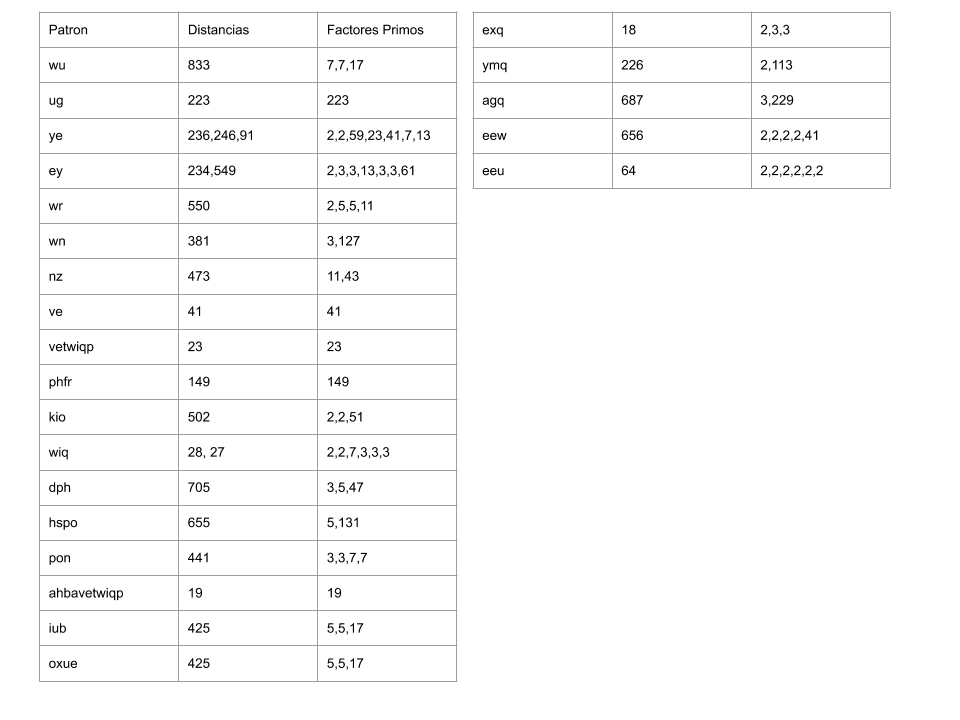
\includegraphics[width=\textwidth]{vigenere}\\

Luego de ellos vemos los factores que más se repiten, encontramos 2, 3. Pero al hacer la prueba con una longitud de palabra clave 6, no obtuvimos ningun resultado coherente.
Así que intentamos con los factores 3, 5 ya que está sería una buena longitud de palabra clave similar a la del ejercicio hecho en clase.\\

Así que partimos el texto en renglones con 15 letras cada una obteniendo lo siguiente:\\
WUGYEYGAWRAWNZV\\
EILJKIOCPLTFEIW\\
IQVWJMDPHSPONAM\\
WGRMZEAAHBAVETW\\
IQPHMIUBUAEEXFE\\
WOXUEXQAHBAVETW\\
IQPNMWJWMAEXQKY\\
MQUJLEOBRAGQPXN\\
SQPGZTGKKOFYNFS\\
VTXYCOCAWAYLBGH\\
EFTOVWQSRCAQDÑI\\
XHEJJVCAHSGQNEE\\
WÑRMJEDIBOFSPTW\\
QHHNLVCXDSTSZYY\\
IHPÑJEIPFOEEUGI\\
XQHHTYAIDBEYEWE\\
JNEOCENWFOXMOIC\\
OBJMRZGKRNQYZWM\\
HBVMZWCABLWEZNS\\
EEUUEGCUSEDSRÑI\\
OBSYGVFMDQGIXEE\\
LUVÑGVKITUPEXYM\\
QPHFRNQZPAOENXO\\
ONWJTETWPLMKEBP\\
EFBMZWCABAXMFIO\\
SXDNCEIZLMMWNKY\\
IYHFGHGKLSWSFXI\\
WYXXRFNMHSMOGTQ\\
IEDSNEOIBCMTEBG\\
LBVURQVMVQGIQEW\\
IZWCDMGUWOOIFÑE\\
OYDVJSVIUAPONZY\\
EPHFRIUBHRTOEIG\\
EOXUEHQTHLAGBGX\\
EERHKIOBLEWJEBS\\
HQXHRLQQDDPEOXV\\
SQPFRWGUWRMRNMP\\
INSJPIEWPTDEQEP\\
YERSMQKUVTMQGXO\\
EORHTMGUFIMTQLH\\
MPHXGQFMHSFEÑTG\\
ELRNGFTMOIPWCBV\\
MGXFRQQKKEPQULE\\
CQPKZIFIGSPEZXK\\
SQÑUCPCGVEXIEXZ\\
IXRKGVSCHSPOXIV\\
ELFJDTTMPDTYZTZ\\
IMSJJUWMVEXEGTT\\
EFRFRQWJHDPHBES\\
VORHHIOIÑORVQUE\\
OÑXWVETJUEHIFJE\\
ONEMRWSCLEYPQWM\\
SXDHGXKKLAGQRBI\\
ONOCXSÑMKAÑMNÑQ\\
KEDHWEXWULPHUEE\\
WSUUTMCA\\

Con lo cual obtenemos 15 columnas por hacer análisis de frecuencias, sobre las cuales vamos obteniendo las letras de la palabra clave.\\

Columna 1 = E\\
Columna 2 = N\\
Columna 3 = D\\
Columna 4 = U\\
Columna 5 = R\\
Columna 6 = E\\
Columna 7 = C\\
Columna 8 = I\\
Columna 9 = D\\
Columna 10 = A\\
Columna 11 = M\\
Columna 12 = E\\
Columna 13 = N\\
Columna 14 = T\\
Columna 15 = E \\

Con lo cual formamos la palabra $\textbf{ENDURECIDAMENTE}$, metemos la palabra clave en el programa de cifrado de vigenere visto en laboratorio. Y vemos que el texto queda descifrado de la siguiente manera:\\

"SIDENUESTROSAGRAVIOSENUNLIBROSEESCRIBIESELAHI\\
STORIAYSEBORRASEENNUESTRASALMASCUANTOSEBORRA\\
SEENSUSHOJASTEQUIEROTANTOAUNDEJOENMIPECHOTU\\
AMORHUELLASTANHONDASQUESOLOCONQUETUBORRASESUN\\
ALASBORRABAYOTODASNUESTRAPASIONFUEUNTRAGICOSAIN\\
ETEENCUYAABSURDAFABULALOCOMICOYLOGRAVECONFUND\\
IDOSRISASYLLANTOARRANCANPEROFUELOPEORDEAQUEL\\
LAHISTORIAQUEALFINDELAJORNADAAELLATOCARONLAGR\\
IMASYRISASYAMISOLOLASLAGRIMASAQUEMELODECISLO\\
SEESMUDABLEESALTANERAYVANAYCAPRICHOSAANTESQUE\\
ELSENTIMIENTODESUALMABROTARAELAGUADELAESTERILR\\
OCACUANDOMELOCONTARONSENTIELFRIODEUNAHOJADEAC\\
EROENLASENTRAÑASMEAPOYECONTRAELMUROYUNINSTANT\\
ELACONCIENCIAPERDIDEDONDEESTABACAYOSOBREMIES\\
PIRITULANOCHEENIRAYENPIEDADSEANEGOELALMAYSEMER\\
EVELOPORQUESELLORAYCOMPRENDIUNAVEZPORQUESEMATAP\\
ASOLANUBEDEDOLORCONPENALOGREBALBUCEARBREVESPALA\\
BRASQUIENMEDIOLANOTICIAUNFIELAMIGOMEHACIAU\\
NGRANFAVORLEDILASGRACIAS"\\
 
\section*{Ejercicio 6}
A partir de la pista otorgada (obteniendo el texto cifrado "NNXRHPZHVTHMGSMIXGJYOYHMDKOE" del texto en claro "NATURALEZA ATÓMICA DE LA MATERIA").\\
\\
NA TU RA LE ZA AT OM IC AD EL AM AT ER IA\\
NN XR HP ZH VT HM GS MI XG JY OY HM DK OE \\
 \\
Se obtienen los siguientes valoreas de acuerdo a la posición de las letras.\\
\\
$
\begin{pmatrix}
N \\ N 
\end{pmatrix}
=
\begin{pmatrix}
13 \\ 13
\end{pmatrix}
\longrightarrow
\begin{pmatrix}
13 \\ 0 
\end{pmatrix}
=
\begin{pmatrix}
N \\ A 
\end{pmatrix}
$\\
%-------------------------1
$
\begin{pmatrix}
X \\ R 
\end{pmatrix}
=
\begin{pmatrix}
23 \\ 17
\end{pmatrix}
\longrightarrow
\begin{pmatrix}
19 \\ 20 
\end{pmatrix}
=
\begin{pmatrix}
T \\ U 
\end{pmatrix}
$\\
%-----------------------------2
$
\begin{pmatrix}
H \\ P 
\end{pmatrix}
=
\begin{pmatrix}
7 \\ 15
\end{pmatrix}
\longrightarrow
\begin{pmatrix}
17 \\ 0 
\end{pmatrix}
=
\begin{pmatrix}
R \\ A
\end{pmatrix}
$\\
%-----------------------------3
$
\begin{pmatrix}
Z \\ H 
\end{pmatrix}
=
\begin{pmatrix}
25 \\ 7
\end{pmatrix}
\longrightarrow
\begin{pmatrix}
11 \\ 4 
\end{pmatrix}
=
\begin{pmatrix}
L \\ E
\end{pmatrix}
$\\
%-----------------------------4
$
\begin{pmatrix}
V \\ T 
\end{pmatrix}
=
\begin{pmatrix}
21 \\ 19
\end{pmatrix}
\longrightarrow
\begin{pmatrix}
25 \\ 0 
\end{pmatrix}
=
\begin{pmatrix}
Z \\ A
\end{pmatrix}
$\\
%-----------------------------5
$
\begin{pmatrix}
H \\ M
\end{pmatrix}
=
\begin{pmatrix}
7 \\ 12
\end{pmatrix}
\longrightarrow
\begin{pmatrix}
0 \\ 19 
\end{pmatrix}
=
\begin{pmatrix}
A \\ T
\end{pmatrix}
$\\
%-----------------------------6
$
\begin{pmatrix}
G \\ S 
\end{pmatrix}
=
\begin{pmatrix}
6 \\ 18
\end{pmatrix}
\longrightarrow
\begin{pmatrix}
14 \\ 12 
\end{pmatrix}
=
\begin{pmatrix}
O \\ M
\end{pmatrix}
$\\
%-----------------------------7
$
\begin{pmatrix}
M \\ I 
\end{pmatrix}
=
\begin{pmatrix}
12 \\ 8
\end{pmatrix}
\longrightarrow
\begin{pmatrix}
8 \\ 2 
\end{pmatrix}
=
\begin{pmatrix}
I \\ C
\end{pmatrix}
$\\
%-----------------------------8
$
\begin{pmatrix}
X \\ G 
\end{pmatrix}
=
\begin{pmatrix}
23 \\ 6
\end{pmatrix}
\longrightarrow
\begin{pmatrix}
0 \\ 3 
\end{pmatrix}
=
\begin{pmatrix}
A \\ D
\end{pmatrix}
$\\
%-----------------------------9
$
\begin{pmatrix}
J \\ Y 
\end{pmatrix}
=
\begin{pmatrix}
9 \\ 24
\end{pmatrix}
\longrightarrow
\begin{pmatrix}
4 \\ 11 
\end{pmatrix}
=
\begin{pmatrix}
E \\ L
\end{pmatrix}
$\\
%-----------------------------10
$
\begin{pmatrix}
O \\ Y 
\end{pmatrix}
=
\begin{pmatrix}
14 \\ 24
\end{pmatrix}
\longrightarrow
\begin{pmatrix}
0 \\ 12 
\end{pmatrix}
=
\begin{pmatrix}
A \\ M
\end{pmatrix}
$\\
%-----------------------------11
$
\begin{pmatrix}
H \\ M 
\end{pmatrix}
=
\begin{pmatrix}
7 \\ 12
\end{pmatrix}
\longrightarrow
\begin{pmatrix}
0 \\ 14 
\end{pmatrix}
=
\begin{pmatrix}
A \\ T
\end{pmatrix}
$\\
%-----------------------------12
$
\begin{pmatrix}
D \\ K 
\end{pmatrix}
=
\begin{pmatrix}
3 \\ 10
\end{pmatrix}
\longrightarrow
\begin{pmatrix}
4 \\ 17 
\end{pmatrix}
=
\begin{pmatrix}
E \\ R
\end{pmatrix}
$\\
%-----------------------------13
$
\begin{pmatrix}
O \\ E 
\end{pmatrix}
=
\begin{pmatrix}
14 \\ 4
\end{pmatrix}
\longrightarrow
\begin{pmatrix}
8 \\ 0 
\end{pmatrix}
=
\begin{pmatrix}
I \\ A
\end{pmatrix}
$\\
%-----------------------------14
\\
Enseguida se procede a buscar los sistemas de ecuaciones más fáciles de resolver, entre estos se encuentra la siguiente relación:


$$
\begin{pmatrix}
H \\ P 
\end{pmatrix}
=
\begin{pmatrix}
7 \\ 15
\end{pmatrix}
\longrightarrow
\begin{pmatrix}
17 \\ 0 
\end{pmatrix}
=
\begin{pmatrix}
R \\ A
\end{pmatrix}
$$\\
\\
La cual nos proporciona el sistema 
\\
$$17a + 0b \equiv 7 \pmod{26}$$
$$17c + 0d \equiv 7 \pmod{26}$$
\\
A partir del cual obtenemos las siguientes:
\\
\begin{equation}
17a \equiv 7 \pmod{26}
\end{equation}
\begin{equation}
17c \equiv 15 \pmod{26}
\end{equation}
\\
Podemos ver que tanto en (1) como en (2), es posible obtener el valor de a y c pues $mcd(7,26)=1$ y $mcd(15,26)=1$
\\
En el caso de (1) tenemos lo siguiente:
\begin{equation}
17x - 26y = 1
\end{equation}
Donde obtenemos que $x=-3$ y $y=-2$, entonces:
$$17(-3)-26(-2)=1$$
Para obtener a, multiplicamos todo por 7 y tenemos:
$$17(-21)-26(-14)=7$$
$$inverso(17) \equiv -21 \pmod{26}$$
$$a = -21 \pmod{26} = 5$$
$$a = 5$$
\\
Si hacemos lo mismo para (2) con la fórmula (3) obtenemos:
$$17(-45)-26(-30)=15$$
$$inverso(17) \equiv -45 \pmod{26}$$
$$c = -45 \pmod{26} = 7$$
$$c = 7$$
Ahora se buscan los valores de b y d, a partir de la relación:
$$
\begin{pmatrix}
J \\ Y 
\end{pmatrix}
=
\begin{pmatrix}
9 \\ 24
\end{pmatrix}
\longrightarrow
\begin{pmatrix}
4 \\ 11 
\end{pmatrix}
=
\begin{pmatrix}
E \\ L
\end{pmatrix}
$$\\
\\
De la cual obtenemos
\\
\begin{equation}
4a + 11b \equiv 9 \pmod{26}
\end{equation}
\begin{equation}
4c + 11d \equiv 24 \pmod{26}
\end{equation}
\\
Si sustituímos el valor de a en (4)
$$4(5) + 11b \equiv 9 \pmod{26} $$
$$20 + 11b \equiv 9 \pmod{26} $$
$$b=25$$
Y por otro lado, hacemos lo mismo con c en (5)
$$4(7) + 11d \equiv 24 \pmod{26} $$
$$28 + 11d \equiv 24 \pmod{26} $$
$$d=2$$
Obteniendo la MATRIZ DE CIFRADO
$$M = 
\begin{pmatrix}
a & b \\
c & d
\end{pmatrix}
=
\begin{pmatrix}
5 & 25 \\
7 & 2
\end{pmatrix}
$$
Entonces se busca la matriz inversa de esta para obtener la MATRIZ DE DESCIFRADO.
Para esto vemos que el determinante de M es 17 y  $mcd(17,23)=1$, entonces sí existe el inverso multiplicativo de $17 \pmod{26}$ el cual es 23.
Entonces:
$$
M^{-1} = \frac{1}{17} 
\begin{pmatrix}
d & -b \\
-c & a
\end{pmatrix}
\pmod{26}
=
23
\begin{pmatrix}
2 & -25 \\
-7 & 5
\end{pmatrix}
\pmod{26}
$$
\\
$$
M^{-1} =
\begin{pmatrix}
20 & 23 \\
21 & 11
\end{pmatrix}
$$
Entonces al descifrar el texto con esta MATRIZ De DESCIFRADO (LLAVE) obtenemos el sieguiente texto:\\
"
LA HIPOTESIS ATOMICA EL CONCEPTO DEL ATOMO EN LA FORMA QUE FUERA ACEPTADO POR LO CIENTIFICOS DESDE MIL SEISCIENTOS DE HASTA MIL NOVECIENTOS SE BASO EN LAS IDEAS DE FILOSOFOS GRIEGOS DEL SIGLO VA FUERON LEUCIPPO DE MILETO Y SU DISCIPULO DEMOCRITO DE ABDERA
QUIENES ORIGINARON LA FILOSOFIA ATOMICA INTRODUCIENDO LA NOCION DE UN CONSTITUYENTE ULTIMO DE LA MATERIA QUE DENOMINARON ATOMO ES DECIR INDIVISIBLE EN LA LENGUA GRIEGA DEMOCRITO CREIA QUE LOS ATOMOS ERAN UNIFORMES SOLIDOS DUROS INCOMPRESIBLES E INDESTRUCTIBLES Y QUE SE MOVIAN EN NUMERO INFINITO POR EL ESPACIO VACIO SEGUN SUS IDEAS LAS DIFERENCIAS DE FORMA Y TAMANO DE LOS ATOMOS DETERMINABAN LAS PROPIEDADES DE LA MATERIA ESTAS ESPECULACIONES FUERON LUEGO CONTINUADAS POR EPICURO DE SAMOSSI BIEN LA TEORIA ATOMICA GRIEGA ES SIGNIFICATIVA DEL PUNTO DE VISTA HISTORICO Y FILOSOFICO CARECE DE VALOR CIENTIFICO PUES NO SE FUNDA EN OBSERVACIONES DE LA NATURALEZA NI EN MEDICIONES PRUEBAS Y EXPERIMENTOS PARA LOS GRIEGOS LA CIENCIA CONSTITUIA TAN SOLO UN ASPECTO DE SU SISTEMA FILOSOFICO MEDIANTE EL CUAL BUSCABAN UNA TEORIA GENERAL QUE EXPLICARA EL UNIVERSO CON ESTE FIN ELLOS USABAN CASI EXCLUSIVAMENTE LA MATEMATICA Y EL RAZONAMIENTO CUANDO HABLABAN DE LA FISICA FUE ASI QUE PLATON Y ARISTOTELES ATACARON LA TEORIA ATOMICA SOBRE BASES FILOSOFICAS Y NO CIENTIFICAS EN EFECTO MIENTRAS DEMOCRITO CREIA QUE LA MATERIA NO SE PODIA MOVER EN EL ESPACIO SIN EL VACIO Y QUE LA LUZ CONSISTIA DEL RAPIDO MOVIMIENTO DE PARTICULAS A TRAVES DEL VACIO PLATON RECHAZABA LA IDEA QUE ATRIBUTOS COMO BONDAD O BELLEZA FUERAN SIMPLEMENTE MANIFESTACIONES MECANICAS DE ATOMOS MATERIALES DEL MISMO MODO ARISTOTELES NO ACEPTABA LA EXISTENCIA DEL VACIO PUES NO PODIA CONCEBIR QUE LOS CUERPOS CAYERAN CON IGUAL RAPIDEZ EN UN VACIO EL PUNTO DE VISTA ARISTOTELICO PREVALECIO EN LA EUROPA MEDIOEVAL Y LA CIENCIA DE LOS TEOLOGOS CRISTIANOS SE BASO EN LA REVELACION Y LA RAZON MOTIVO POR EL CUAL LAS IDEAS DE DEMOCRITO FUERON REPUDIADAS POR CONSIDERARSE LAS MATERIALISTAS Y ATEAS"


\end{document}

